\documentclass[
oneside,
fontsize=11pt
]{scrartcl}



%%%%%%%%%%%%%%%%%%%%%%%%%%%%%%%%%%%%%%%%%%%%%%%%%%%%%%%%%%%%%%%%%%%%%%%%%%%%%%%%
%%%
%%% packages
%%%

%%%
%%% encoding and language set
%%%


\usepackage[english]{babel}
\usepackage[a4paper]{geometry}

%%% fontenc, ae, aecompl: coding of characters in PDF documents
\usepackage[utf8]{inputenc}
\usepackage[T1]{fontenc}
\usepackage{lmodern}

\usepackage[autostyle=true,german=quotes]{csquotes}
\usepackage{caption}
\usepackage{subcaption}
\usepackage{minted}

%%%
%%% technical packages
%%%

% \usepackage{svg}

%%% pgf plots from matplotlib tikzplotlib
\usepackage{pgfplots}
\DeclareUnicodeCharacter{2212}{−}
\usepgfplotslibrary{groupplots,dateplot}
\usetikzlibrary{patterns,shapes.arrows}
\pgfplotsset{compat=newest}

%%% amsmath, amssymb, amstext: support for mathematics
\usepackage{amsmath,amssymb,amstext}


%%%
%%% Colors
%%%
\definecolor{TUGreen}{rgb}{0.517,0.721,0.094}


%%%
%%% Macros
%%%
\newtheorem{mydef}{Definition}
\newcommand{\mydefautorefname}{Definition}



\usepackage{graphicx}

%%% hyperref (hyperlinks in PDF): for more options or more detailed
%%%          explanations, see the documentation of the hyperref-package
\usepackage[%
  %%% general options
  pdftex=true,      %% sets up hyperref for use with the pdftex program
  %plainpages=false, %% set it to false, if pdflatex complains: ``destination with same identifier already exists''
  %
  %%% extension options
  backref,      %% adds a backlink text to the end of each item in the bibliography
  pagebackref=false, %% if true, creates backward references as a list of page numbers in the bibliography
  colorlinks=true,   %% turn on colored links (true is better for on-screen reading, false is better for printout versions)
  linkcolor=TUGreen,
  urlcolor=TUGreen,
  %
  %%% PDF-specific display options
  bookmarks=true,          %% if true, generate PDF bookmarks (requires two passes of pdflatex)
  bookmarksopen=true,     %% if true, show all PDF bookmarks expanded
  bookmarksnumbered=true, %% if true, add the section numbers to the bookmarks
  %pdfstartpage={1},        %% determines, on which page the PDF file is opened
  pdfpagemode=None         %% None, UseOutlines (=show bookmarks), UseThumbs (show thumbnails), FullScreen
]{hyperref}


%%% sets the PDF-Information options
%%% (see fields in Acrobat Reader: ``File -> Document properties -> Summary'')
%%% Note: this method is better than as options of the hyperref-package (options are expanded correctly)
\hypersetup{
  pdftitle={Fréchet Distance}, %%
  pdfauthor={Tom Stein}, %%
  pdfsubject={Seminar Algorithm Engineering 22/23}, %%
  pdfcreator={Accomplished with LaTeX2e and pdfLaTeX with hyperref-package.}, %% 
  pdfproducer={}, %%
  pdfkeywords={} %%
}



%%%%%%%%%%%%%%%%%%%%%%%%%%%%%%%%%%%%%%%%%%%%%%%%%%%%%%%%%%%%%%%%%%%%%%%%%%%%%%%%
%%%
%%% define the titlepage
%%%

% \subject{}   %% subject which appears above titlehead
% \titlehead{} %% special heading for the titlepage

%%% title
\title{Fréchet Distance}

%%% author(s)
\author{Tom Stein}

%%% date
\date{December 26, 2022}


%%%%%%%%%%%%%%%%%%%%%%%%%%%%%%%%%%%%%%%%%%%%%%%%%%%%%%%%%%%%%%%%%%%%%%%%%%%%%%%%
%%%
%%% begin document
%%%

\begin{document}

% \pagenumbering{roman} %% small roman page numbers

%%% include the title
% \thispagestyle{empty}  %% no header/footer (only) on this page
%  \maketitle

% Titlepage ---------------------------------------------------------
%
\pdfbookmark{Titelpage}{pdf:title}
\newgeometry{
    a4paper,
    top=25mm,
    bottom=25mm,
    left=20mm,
    right=20mm,
}
\begin{titlepage}
    
\includegraphics[width=0.4\textwidth]{images/tud_logo_rgb.jpg}

    \begin{center}
        \vspace{3.5cm} \LARGE Seminar Algorithm Engineering 22/23

        \vspace{0.5cm} \huge \textbf{Fréchet Distance}

        \vspace{5cm} \textbf{Tom Stein}

        \vspace{0.25cm} \Large December 05, 2022
    \end{center}

    \vspace{5.2cm} \large \noindent Supervisor: \\
    Dr. Carolin Rehs
    
    \vspace{1cm} \noindent Technische Universität Dortmund \\
    Department of Computer Science \\
    Chair 11 (Algorithm Engineering) \\ 
    \url{https://ls11-www.cs.tu-dortmund.de/}

    
\end{titlepage}



%%% start a new page and display the table of contents
% \newpage
% \tableofcontents

%%% start a new page and display the list of figures
% \newpage
% \listoffigures

%%% start a new page and display the list of tables
% \newpage
% \listoftables

%%% display the main document on a new page 
\newpage

% \pagenumbering{arabic} %% normal page numbers (include it, if roman was used above)
 
%%%%%%%%%%%%%%%%%%%%%%%%%%%%%%%%%%%%%%%%%%%%%%%%%%%%%%%%%%%%%%%%%%%%%%%%%%%%%%%%
%%%
%%% begin main document
%%% structure: \section \subsection \subsubsection \paragraph \subparagraph
%%%

\newgeometry{left=3cm, right=4cm, top=3cm, bottom=3cm}

\section*{Abstract}
% The Fréchet distance is a metric used to compare curves in a metric space
% that takes the course of the curves into account.
% This report will give an overview on the Fréchet distance 
% covering the general motivation, 
% the formal definition along with easy to understand explanations, 
% the weak and discrete variants, and algorithms to compute all of them.

The Fréchet distance is a metric used to compare curves in a metric space. 
It measures the similarity between two curves based on the overall shape and course of the curves. 
This report will provide an overview of the Fréchet distance, 
including its formal definition, weak and discrete variants, and algorithms for efficiently computing the distance. 
The report will also cover the general motivation for using the Fréchet distance 
and its applications in fields such as pattern recognition, computer vision, and geographic information systems. 
The report is structured to provide a comprehensive understanding of the Fréchet distance, 
including easy-to-understand explanations 
and a discussion of trade-offs between computational complexity and accuracy in the algorithms for computing the distance.


\section{Introduction}
% motivation
At first, it seems that measuring the similarity between two curves
is a very theoretical problem, but it has many, not that obvious, practical applications.
It is used in geographic information systems (GIS) to 
quantify the similarity or quality of two maps \cite{lyu_partial-frechet-distance-based_2022},
find patterns in vehicle traffic or animal tracking data 
by trajectory analysis \cite{buchin_detecting_2011},
gesture recognition on touch devices like smartphones \cite{hu_research_2022},
and shape matching in the field of computer vision. 

To quantify the similarity of two given curves (e.g. shapes, paths, or trajectories)
a distance metric can be used. 
We can not simply use a distance metric like euclidean distance 
because we do not want to compare points to points 
but instead compare curves to curves. 
Therefore, we start by defining curves in \autoref{def_curve}.

% two (polygonal) curves
% TODO: replace continous funcitons with other name
\begin{mydef}
  \label{def_curve}
  We define a curve as a continuous function $f : [a,b] \mapsto V$ 
  with $a,b \in \mathbb{R}, a \leq b$ and $V$ being the space of the curve,
  e.g., $\mathbb{R}^2$ or $\mathbb{R}^3$.
\end{mydef}

\begin{mydef}
  \label{def_polygonal_curve}
  We define a polygonal curve (polygonal chain) 
  as a linearly interpolated curve 
  on $n \in \mathbb{N}$ points in $V$.
  Therefore, $P : [0,n] \mapsto V$ 
  should be affine on the interval $[i,i+1]$ for all $i \in \{0, 1, \dots, n-1\}$, 
  i.e., $P(i + \lambda) = (1 - \lambda)P(i) + \lambda P(i+1)$ for all $\lambda \in [0,1]$.
\end{mydef}

In the following we will focus on polygonal curves (polygonal chains) 
as defined in \autoref{def_polygonal_curve} 
instead of classical curves (\autoref{def_curve}), often used in pure mathematics, 
because most data we have in this area is 
captured by some noncontinuous mechanism, e.g., GPS positions from a tracking device.
Additionally, we focus on the 2D Space, i.e. $V = \mathbb{R}^2$.
However, many concepts also apply to normal curves and higher dimensional spaces.


% Hausdorff distance
The commonly known \textit{Hausdorff distance} can be understood 
as the largest distance between any two points on the curves. 
For each curve, a point with the maximum shortest distance to a point on the other curve is searched for, see \autoref{fig_hausdorff_distance_example}. \cite{alt_computing_1995}


\begin{mydef}
  \label{def_hausdorff_distance}
  Given two normal or polygonal curves $P$ and $Q$, 
  their Hausdorff distance $\delta_{hd}(P,Q)$ is defined as: 
  $$\delta_{hd}(P,Q) = \max \left( \sup_{p \in P} \inf_{q \in Q} \text{dist}(p,q), \sup_{q \in Q} \inf_{p \in P} \text{dist}(p,q) \right)$$
\end{mydef}

The Hausdorff distance metric $\delta_{hd}(P,Q)$ defined in \autoref{def_hausdorff_distance} 
is very intuitive and can be easily computed for polygonal curves \cite{ko_complexity_2013}.
It finds applications in computer vision and computer graphics 
where it is used to compare the similarity of two mesh objects \cite{cignoni_metro_1998,ko_complexity_2013}. 
However, this metric does not take the course of the curves into account, 
but only the point sets of the individual curves.
Two curves may have a small Hausdorff distance but seem very dissimilar 
when looking at them, see \autoref{fig_hausdorff_distance_bad_example}.

\begin{figure}[ht]
  \centering
  \begin{subfigure}[b]{0.45\textwidth}
      \resizebox{\textwidth}{!}{
        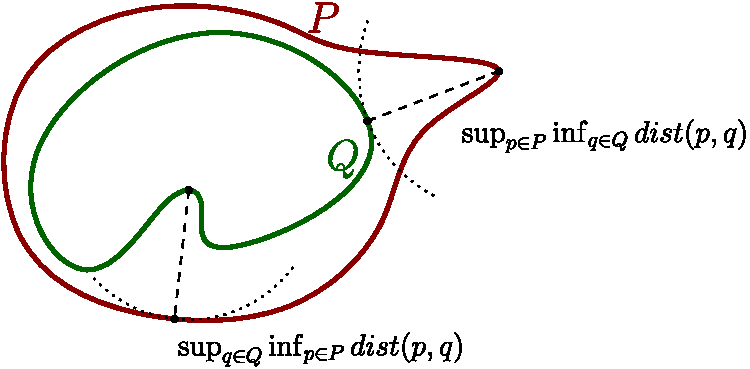
\includegraphics[width=\textwidth]{images/hausdorff/hausdorff-distance-example.pdf}
      }
      \caption{Hausdorff distance between the red curve $P$ and green curve $Q$. }
      \label{fig_hausdorff_distance_example}
  \end{subfigure}
  \hfill
  \begin{subfigure}[b]{0.45\textwidth}
      \resizebox{\textwidth}{!}{
        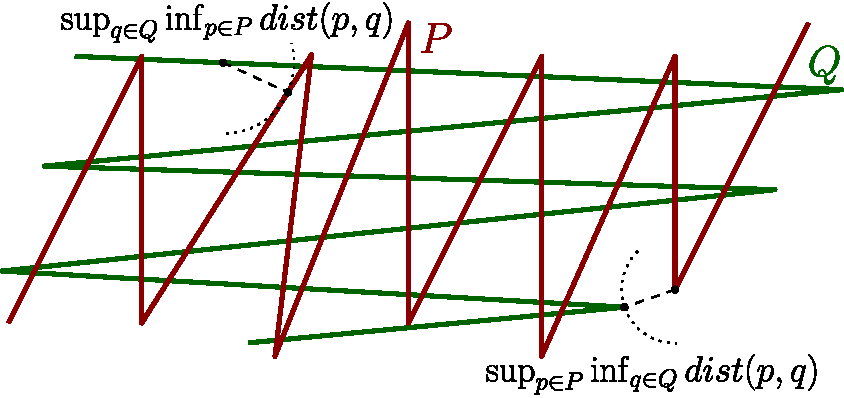
\includegraphics[width=\textwidth]{images/hausdorff/hausdorff-distance-bad-example.pdf}
      }
      \caption[Hausdorff distance of two dissimilar curves]{Two dissimilar curves with a small Hausdorff distance.}
      \label{fig_hausdorff_distance_bad_example}
  \end{subfigure}
  \caption[Hausdorff distance examples]{Hausdorff distance examples.}
  \label{fig_hausdorff_distance_examples}
\end{figure}


% Fréchet distance motivation
In reality, the course of the curves is important for many applications. 
For example, 
in handwriting character recognition on digital input devices, especially in Chinese \cite{chanin_david_hanzi_nodate},
(online) handwriting signature verification \cite{zheng_algorithm_2008,fang_research_2018},
gesture recognition on smartphone touchscreens \cite{hu_research_2022}, % TODO: add more citations
map-matching tracking data for traffic control, routing and navigation \cite{wenk_addressing_2006,brakatsoulas_map-matching_2005},
moving object analysis, e.g., detecting commuting patterns \cite{buchin_detecting_2011},
and motion evaluation in real-time motion capturing \cite{qiao_real-time_2017, shehu_curve_2012}. % TODO: add more citations
For this reason, the \textit{Fréchet distance}, named after the famous French mathematician René Maurice Fréchet, was introduced.

A common analogy for the Fréchet distance can be shown by a man walking his dog. 
Assume that both the man and the dog are moving along a predefined fixed curve. 
Both are free to adjust their speed as they wish, even to stop. 
However, they are not allowed to go backwards. 
We are looking for the minimum length of the dog leash 
that is necessary for both of them to reach their destination. 
The length of the dog leash is then exactly the Fréchet distance of the two curves.
A formal definition is given in \autoref{def_frechet_distance} 
along with a visual example in \autoref{fig_frechet_distance_example}.

% continuous Fréchet distance equation
\begin{mydef}
  \label{def_frechet_distance}
  Given two (polygonal) curves $P: [a,a'] \mapsto V$, $Q: [b,b'] \mapsto V$ and a distance function $\text{dist}: (V,V) \mapsto \mathbb{R}$, 
  their Fréchet distance $\delta_{F}(P,Q)$ is defined as: 
  $$\delta_{F}(P,Q) = \inf_{\substack{\alpha: [0,1] \mapsto [a, a'] \\ \beta: [0,1] \mapsto [b, b']}} \max_{t \in [0,1]} \text{dist}(P(\alpha(t)), Q(\beta(t)))$$
  where $\alpha$ and $\beta$ represent the walking speed as 
  continuous monotonically increasing functions with
  $\alpha(0) = a, \alpha(1) = a'$, 
  $\beta(0) =b, \beta(1) =b'$.
\end{mydef}

\begin{figure}[ht]
  \centering
  % TODO: Add example graphic of Frechet distance
  % 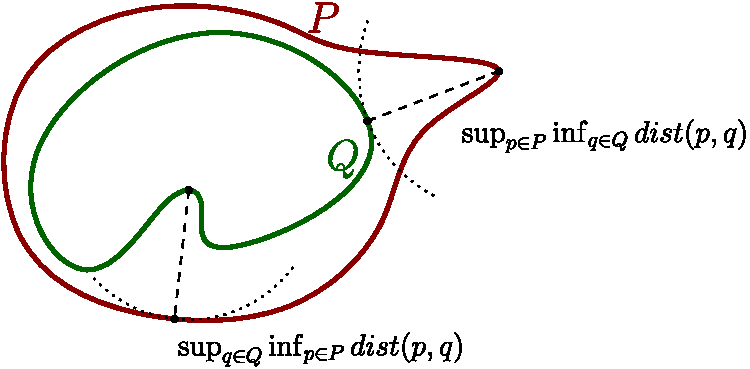
\includegraphics[width=\textwidth]{images/hausdorff/hausdorff-distance-example.pdf}
  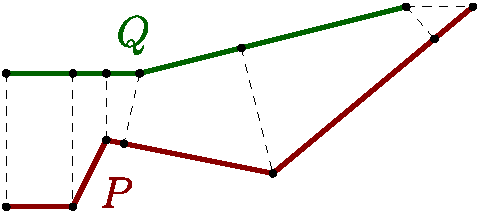
\includegraphics{images/frechet_distance/frechet-distance-example.pdf}
  \caption{The Fréchet distance is indicated by the black lines connecting the two polygonal curves.}
  \label{fig_frechet_distance_example}
\end{figure}



% Scope
% - Different Variants and their differences
% - Original Algorithm by Alt and Godau
% - Original Algorihm for discrete Fréchet distance
% - Newer Algorithms (vor variants)



% Fréchet distance Variants 
\section{Variants}
Through the years many slightly different variants of the continuous Fréchet distance (see Definition \ref{def_frechet_distance}) have evolved. 
The continuous Fréchet distance takes into account every single point on the curves 
without allowing to walk backwards 
and without any obstacles in between the two curves.
In this chapter the most prominent variants of the Fréchet distance are shortly described 
while algorithms for these are given in the following \autoref{sec_algorithms}.

\subsection{Weak Fréchet Distance}
\label{sec_weak_frechet_distance}
The \textit{weak Fréchet distance} (non-monotone Fréchet distance) 
slightly modifies the continuous version by allowing to go backwards. 
The definition remains the same as for the continuous Fréchet distance in \autoref{def_frechet_distance}
where the monotonicity of $\alpha$ and $\beta$ is no longer required.
Note that they are still required to be continuous and have the correct starting and ending values.
% TODO: Add use cases
The weak Fréchet distance is a lower bound on the continuous Fréchet distance.
However, the ratio between them may be arbitrarily large, 
as can be seen by the structure given in \autoref{fig_weak_frechet_distance}. \cite{alt_computing_1995}

\begin{figure}[ht]
  \centering
  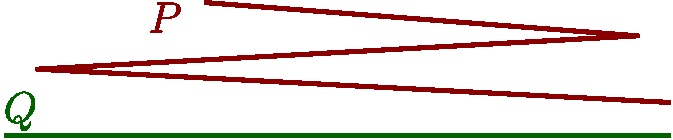
\includegraphics[width=0.8\textwidth]{images/frechet_distance/weak-frechet-distance-example.pdf}
  \caption{
    The two shown polygonal curves $P$ and $Q$ have a small weak Fréchet distance 
    because the point on $Q$ can be moved forward and backward as often as needed. 
    The continuous Fréchet distance is rather large 
    because the point on $Q$ can only move forward.}
  \label{fig_weak_frechet_distance}
\end{figure}



% Discrete Fréchet distance
\subsection{Discrete Fréchet Distance}
The \textit{discrete Fréchet distance} is specifically tied to 
polygonal curves (\autoref{def_polygonal_curve}) 
because it requires a finite number of vertices 
and forbids walking or staying in between them.
The dog walking analogy can be adapted by replacing both the man and the dog by two frogs,
which are only allowed to jump from their current vertex to their next 
vertex in forward direction \cite{bringmann_why_2014}.
While it is allowed for both frogs to jump simultaneously,
it is not allowed to skip vertices while jumping. 
We ensure this behavior by defining a coupling between the curves in \autoref{def_point_coupling}.

\begin{mydef}
  \label{def_point_coupling}
  A \textit{coupling} L between two polygonal curves $P$ and $Q$, 
  with points $(u_1, \dots, u_p)$ and $(v_1, \dots, v_q)$ respectively, 
  is defined as a sequence
  $$(u_{a_1}, v_{b_1}),(u_{a_2}, v_{b_2}), \dots, (u_{a_m}, v_{b_m})$$
  such that $a_1 = 1, b_1 = 1, a_m = p, b_m = q$ 
  while preserving order and the jump length limitation.
  % Note different definiton than in original paper
  % fixes error for unequal length polygonal curves
  Thus, for all $i \in \{1, \dots m-1\}$
  the jump length should be positive but no more than 1,
  i.e., $0 \leq a_{i+1} - a_i \leq 1$ (respectively $0 \leq b_{i+1} - b_i \leq 1$).
\end{mydef}

Note that $P$ and $Q$ may be different in terms of number of points,
implying that the frog on the shorter curve 
has to stop and wait on at least one vertex once
due to the pigeonhole principle.
To order the possible couplings between $P$ and $Q$ we define the 
\textit{length} of a coupling in \autoref{def_coupling_length}. 

\begin{mydef}
  \label{def_coupling_length}
  The \textit{length} $||L||$ of a coupling $L$ is the greatest distance of the $m$ pairs in $L$, that is, 
  $$||L|| = \max_{i=1, \dots, m} dist(u_{a_i}, v_{b_i})$$
\end{mydef}

The definition of the discrete Fréchet distance immediately follows from 
the length of a coupling and is given by \autoref{def_discrete_frechet_distance}.

\begin{mydef}
  \label{def_discrete_frechet_distance}
  Given two polygonal curves $P$ and $Q$
  their discrete Fréchet distance $\delta_{dF}(P,Q)$ is defined as the shortest coupling between them: 
  $$\delta_{dF}(P,Q) = \min \left\{ ||L|| \ | \  L \text{ is a coupling between P and Q} \right\}$$
\end{mydef}

The discrete variant (\autoref{def_discrete_frechet_distance}) gives an upper bound on the continuous Fréchet distance (\autoref{def_frechet_distance}). 
% Clearify if this is really an upper bound for polygonal curves with example
This might not be very obvious for the case of polygonal curves, 
but \autoref{fig_frechet_distance_upper_bound_example} gives an intuitive example.

\begin{figure}[ht]
  \centering
  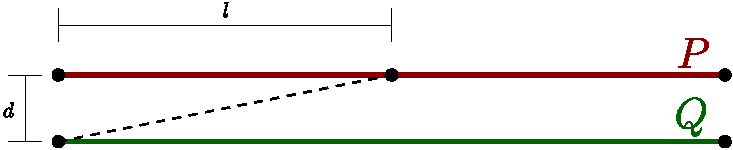
\includegraphics[width=0.8\textwidth]{images/frechet_distance/discrete-frechet-distance-upper-bound.pdf}
  \caption[Upper bound on Fréchet distance]{
    In the case of the discrete Fréchet distance 
    one frog has to wait at either start or end of $Q$
    while the other one is at the middle vertex of $P$, 
    thus requiring a minimal length of $\sqrt{d^2 + l^2}$ for any coupling.
    In contrast, a leash of length $d$ is sufficient for the continuous Fréchet distance.}
  \label{fig_frechet_distance_upper_bound_example}
\end{figure}




Additionally, it is also a lower bound on the continuous Fréchet distance 
plus the distance of the longest legal jump of any frog. 
By increasing the number of points of a polygonal curve that 
overapproximates some other polygonal curve
this property can be used to compute the continuous Fréchet distance \cite{eiter_computing_1994}.

% discrete Fréchet distance and contrast to hausdorff distance
% The discrete Fréchet distance also assings each point another point on the other curve
% just like the hausdorff distance, however it additionally preserves the order of points.

% (Geodesic Fréchet distance)

% (Homotopic Fréchet distance)

% \subsection{Fréchet distance with speed limits}

% \subsection{Fréchet Distance for Uncertain Curves}

\section{Algorithms}
\label{sec_algorithms}
% Chapter summary and structure
Several algorithms to compute the Fréchet distance of polygonal curves were proposed, 
starting from the original algorithm for the continuous variant by Alt and Godau in 1995 \cite{alt_computing_1995}.
The algorithm is based on a concept called free-space diagram and gives a baseline for newer improved versions, 
e.g., the version by Buchin et al. \cite{buchin_four_2017}. 
This chapter is structured as follows: 
first the original algorithm for the continuous Fréchet distance is described in \autoref{sec_original_algorithm}.
% then in \autoref{sec_improved_algorithm} a more recent improved algorithm for the same problem is given.
Afterwards, the modifications necessary to compute the weak variant are described in \autoref{sec_weak_algorithm}.
Finally, an algorithm to compute the discrete Fréchet distance is given in \autoref{sec_discrete_algorithm}.


\subsection{Original Algorithm for the Continuous Fréchet Distance}
\label{sec_original_algorithm}
The original algorithm to compute the continuous Fréchet distance (\autoref{def_frechet_distance})
is based on the idea of solving a simpler decision problem and then doing a parameter search to find the exact value of $\delta_{F}$.
The decision problem is to decide whether two polygonal curves $P$ and $Q$ have a 
Fréchet distance $\delta_{F}(P,Q) \leq \varepsilon$ for some fixed $\varepsilon \geq 0$.

We start by looking at the simplest case for two polygonal curves with two vertices each, i.e., two line segments.
The free space is the set of all valid combinations of positions on $P$ and $Q$ that have a distance of at most $\varepsilon$.
Therefore, we define $F_\varepsilon = \{(s,t) \in [0,1]^2 \ | \ dist(P(s), Q(t)) \leq \varepsilon \}$.
Plotting $s$ and $t$ on a two-dimensional graph, while indicating all illegal combinations in 
another color, gives the free space diagram, see \autoref{fig_free_space}. \cite{alt_computing_1995}

% Free Space Diagram
\begin{figure}[ht]
  \centering
  \begin{subfigure}[b]{0.45\textwidth}
      \resizebox{\textwidth}{!}{
        % 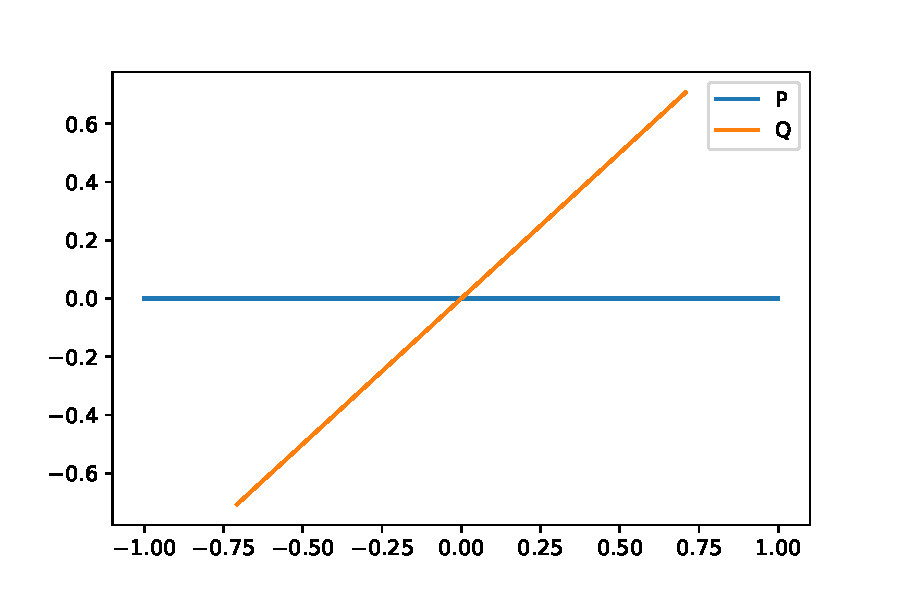
\includegraphics[width=\textwidth]{images/frechet_distance/line_segments.pdf}
        % This file was created with tikzplotlib v0.10.1.
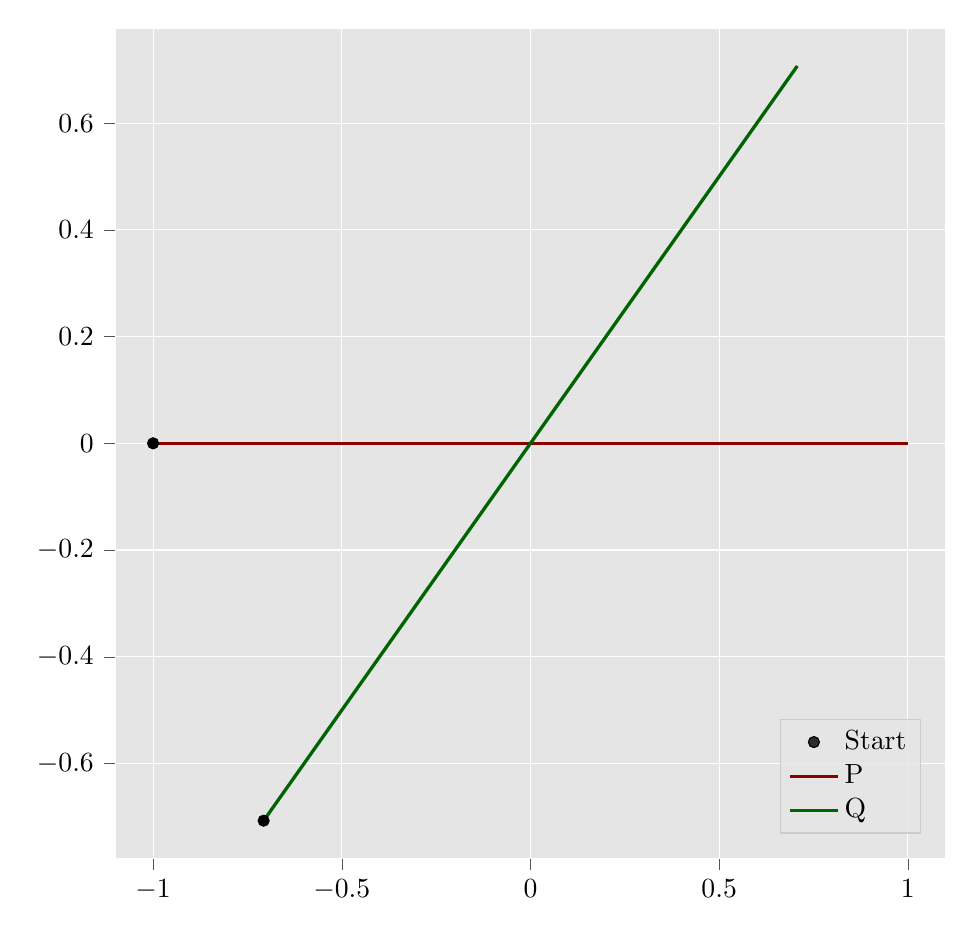
\begin{tikzpicture}

\definecolor{darkgreen}{RGB}{0,100,0}
\definecolor{darkred}{RGB}{139,0,0}
\definecolor{dimgray85}{RGB}{85,85,85}
\definecolor{gainsboro229}{RGB}{229,229,229}
\definecolor{lightgray204}{RGB}{204,204,204}

\begin{axis}[
axis background/.style={fill=gainsboro229},
axis line style={white},
height=\textwidth,
legend cell align={left},
legend style={
  fill opacity=0.8,
  draw opacity=1,
  text opacity=1,
  at={(0.97,0.03)},
  anchor=south east,
  draw=lightgray204,
  fill=gainsboro229
},
minor xtick={},
minor ytick={},
tick align=outside,
tick pos=left,
width=\textwidth,
x grid style={white},
xmajorgrids,
xmin=-1.1, xmax=1.1,
xtick style={color=dimgray85},
xtick={-1.5,-1,-0.5,0,0.5,1,1.5},
y grid style={white},
ymajorgrids,
ymin=-0.777817459305202, ymax=0.777817459305202,
ytick style={color=dimgray85},
ytick={-0.8,-0.6,-0.4,-0.2,0,0.2,0.4,0.6,0.8}
]
\addplot [draw=black, fill=black, mark=*, only marks]
table{%
x  y
-1 0
-0.707106781186548 -0.707106781186547
};
\addlegendentry{Start}
\addplot [very thick, darkred]
table {%
-1 0
1 0
};
\addlegendentry{P}
\addplot [very thick, darkgreen]
table {%
-0.707106828689575 -0.707106828689575
0.707106828689575 0.707106828689575
};
\addlegendentry{Q}
\end{axis}

\end{tikzpicture}

      }
      \caption{Line segments $P$ and $Q$.}
      \label{fig_free_space_lines_example}
  \end{subfigure}
  \hfill
  \begin{subfigure}[b]{0.45\textwidth}
      \resizebox{\textwidth}{!}{
        % 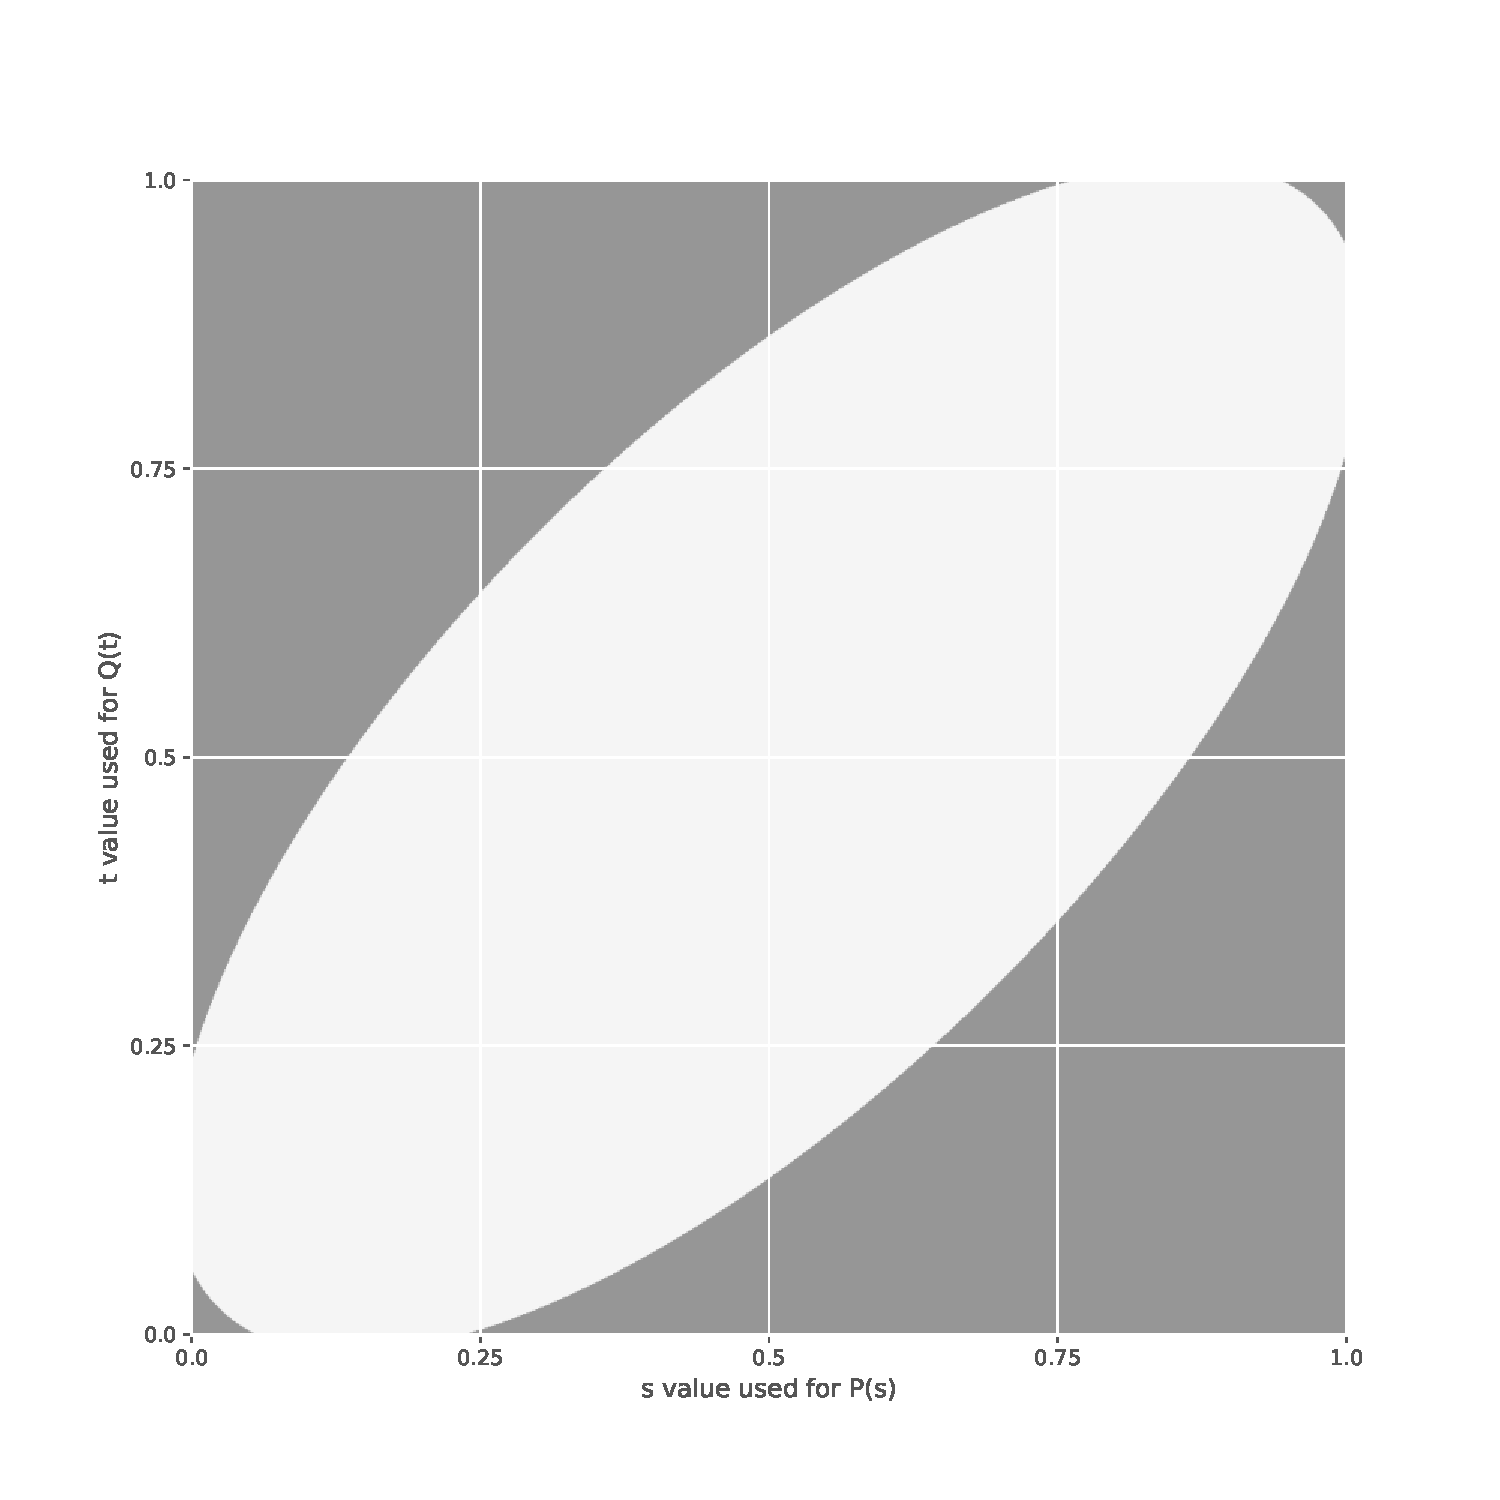
\includegraphics[width=\textwidth]{images/frechet_distance/free_space_single_cell.pdf}
        % This file was created with tikzplotlib v0.10.1.
\begin{tikzpicture}

\definecolor{dimgray85}{RGB}{85,85,85}
\definecolor{gainsboro229}{RGB}{229,229,229}

\begin{axis}[
axis background/.style={fill=gainsboro229},
axis line style={white},
height=\textwidth,
minor xtick={},
minor ytick={},
tick align=outside,
tick pos=left,
width=\textwidth,
x grid style={white},
xlabel=\textcolor{dimgray85}{s value used for P(s)},
xmajorgrids,
xmin=-0.5, xmax=1000,
xtick style={color=dimgray85},
xtick={0,250,500,750,1000},
xticklabels={0.0,0.25,0.5,0.75,1.0},
y grid style={white},
ylabel=\textcolor{dimgray85}{t value used for Q(t)},
ymajorgrids,
ymin=-0.5, ymax=1000,
ytick style={color=dimgray85},
ytick={0,250,500,750,1000},
yticklabels={0.0,0.25,0.5,0.75,1.0}
]
\addplot graphics [includegraphics cmd=\pgfimage,xmin=-0.5, xmax=999.5, ymin=999.5, ymax=-0.5] {images/frechet_distance/free_space_single_cell_image.png};
\end{axis}

\end{tikzpicture}

      }
      \caption{Free space diagram.}
      \label{fig_free_space_diagram_example}
  \end{subfigure}
  \caption[Free space diagram example]{
    The free space diagram \autoref{fig_free_space_diagram_example} 
    for line segments $P$ and $Q$ and distance $\varepsilon = 0.73$
    from \autoref{fig_free_space_lines_example} using euclidean distance.}
  \label{fig_free_space}
\end{figure}

The free space $F_\varepsilon$ has different shapes depending on the employed distance metric,
e.g.,  the intersection of the unit square with an ellipse for euclidean distance 
and with a parallelogram for $L_1$ or $L_\infty$. 
The exact structure of the free space is not further relevant, 
because only the convexity of the area is important. \cite{alt_computing_1995}

We can now extend the free space diagram to longer polygonal curves 
as stated in \autoref{def_free_space}.
An example for a free space diagram on two non-trivial polygonal curves is given in \autoref{fig_complex_free_space}.

\begin{mydef}
  \label{def_free_space}
  Given two polygonal curves $P$ and $Q$ with $p,q \in \mathbb{N}$ vertices respectively, 
  the free space is defined as:
  $$F_\varepsilon = \left\{ (s,t) \in [0,p] \times [0,q] \ | \ dist(P(s), Q(t)) \leq \varepsilon \right\}$$
\end{mydef}

\begin{figure}[ht]
  \centering
  \begin{subfigure}[b]{0.45\textwidth}
      \resizebox{\textwidth}{!}{
        % 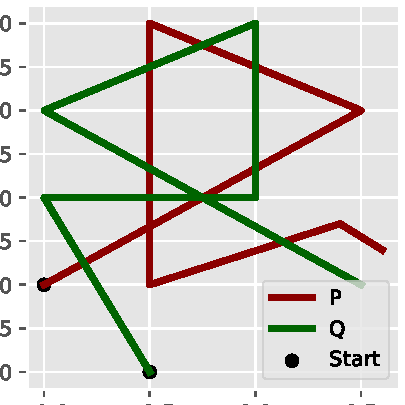
\includegraphics[width=\textwidth]{images/frechet_distance/polygonal_curves.pdf}
        % This file was created with tikzplotlib v0.10.1.
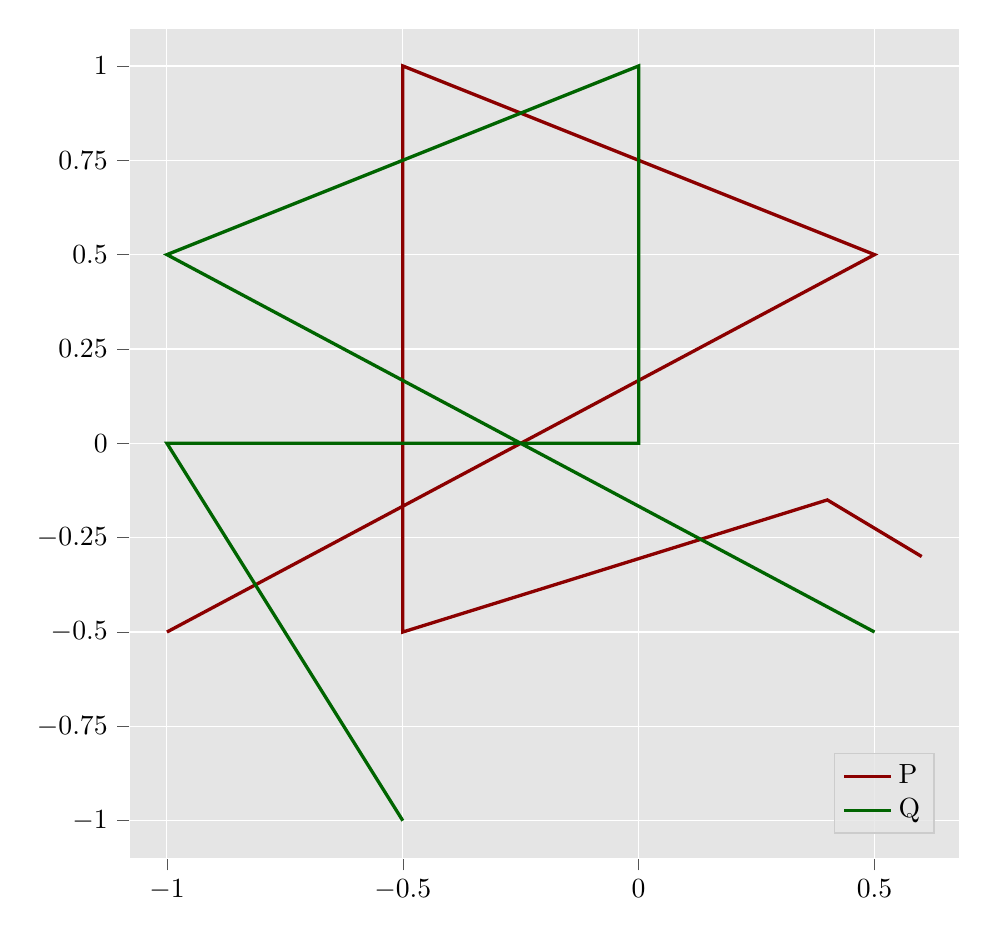
\begin{tikzpicture}

\definecolor{darkgreen}{RGB}{0,100,0}
\definecolor{darkred}{RGB}{139,0,0}
\definecolor{dimgray85}{RGB}{85,85,85}
\definecolor{gainsboro229}{RGB}{229,229,229}
\definecolor{lightgray204}{RGB}{204,204,204}

\begin{axis}[
axis background/.style={fill=gainsboro229},
axis line style={white},
height=\textwidth,
legend cell align={left},
legend style={
  fill opacity=0.8,
  draw opacity=1,
  text opacity=1,
  at={(0.97,0.03)},
  anchor=south east,
  draw=lightgray204,
  fill=gainsboro229
},
minor xtick={},
minor ytick={},
tick align=outside,
tick pos=left,
width=\textwidth,
x grid style={white},
xmajorgrids,
xmin=-1.08, xmax=0.68,
xtick style={color=dimgray85},
xtick={-1.5,-1,-0.5,0,0.5,1},
y grid style={white},
ymajorgrids,
ymin=-1.1, ymax=1.1,
ytick style={color=dimgray85},
ytick={-1.25,-1,-0.75,-0.5,-0.25,0,0.25,0.5,0.75,1,1.25}
]
\addplot [very thick, darkred]
table {%
-1 -0.5
0.5 0.5
-0.5 1
-0.5 -0.5
0.399999976158142 -0.149999976158142
0.600000023841858 -0.299999952316284
};
\addlegendentry{P}
\addplot [very thick, darkgreen]
table {%
-0.5 -1
-1 0
0 0
0 1
-1 0.5
0.5 -0.5
};
\addlegendentry{Q}
\end{axis}

\end{tikzpicture}

      }
      \caption{Polygonal curves $P$ and $Q$.}
      \label{fig_complex_free_space_lines_example}
  \end{subfigure}
  \hfill
  \begin{subfigure}[b]{0.45\textwidth}
      \resizebox{\textwidth}{!}{
        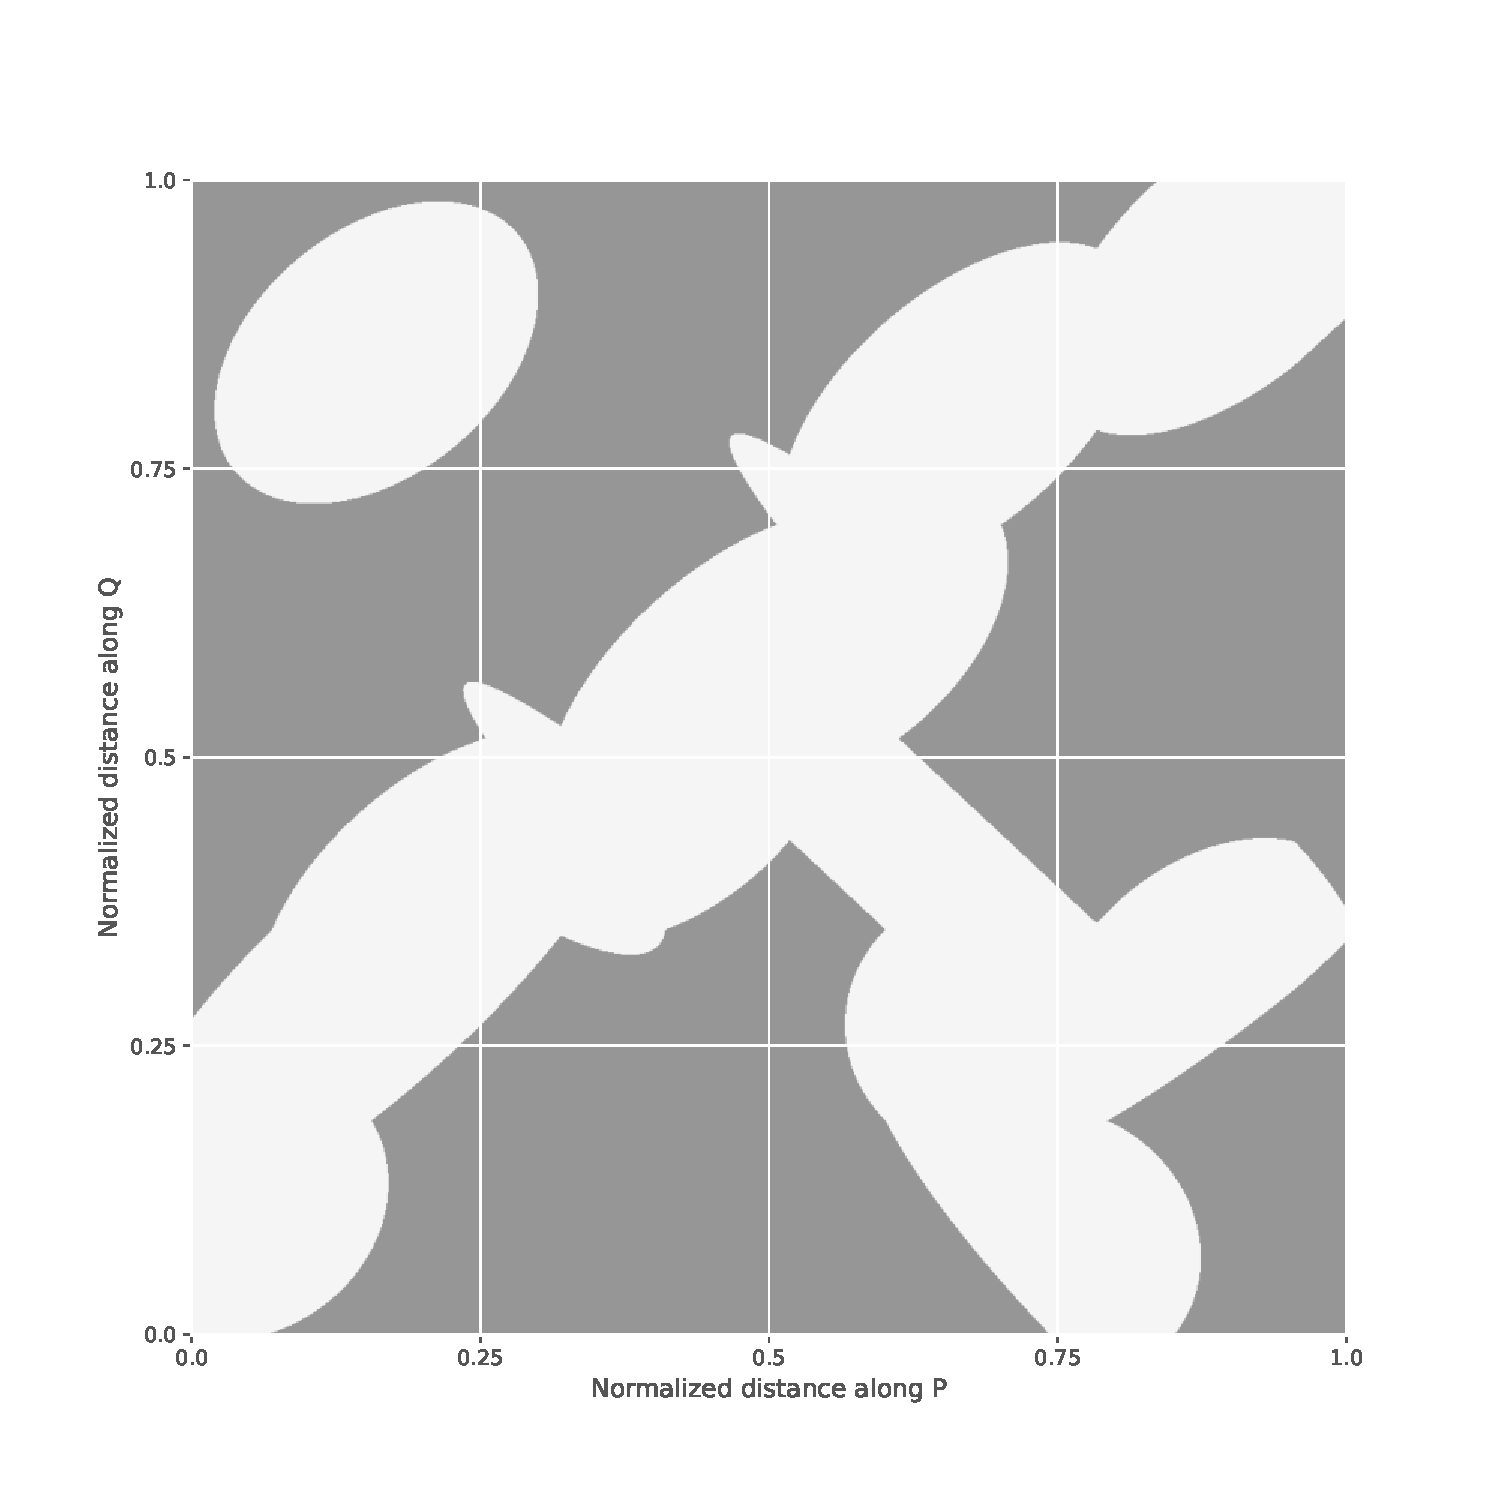
\includegraphics[width=\textwidth]{images/frechet_distance/free_space_polygonal_curves.pdf}
        % % This file was created with tikzplotlib v0.10.1.
\begin{tikzpicture}

\definecolor{dimgray85}{RGB}{85,85,85}
\definecolor{gainsboro229}{RGB}{229,229,229}

\begin{axis}[
axis background/.style={fill=gainsboro229},
axis line style={white},
height=\textwidth,
minor xtick={},
minor ytick={},
tick align=outside,
tick pos=left,
width=\textwidth,
x grid style={white},
xlabel=\textcolor{dimgray85}{s value used for P(s)},
xmajorgrids,
xmin=-0.5, xmax=4995.5,
xtick style={color=dimgray85},
xtick={0,999,1998,2997,3996,4995},
xticklabels={0,1,2,3,4,5},
y grid style={white},
ylabel=\textcolor{dimgray85}{t value used for Q(t)},
ymajorgrids,
ymin=-0.5, ymax=4995.5,
ytick style={color=dimgray85},
ytick={0,999,1998,2997,3996,4995},
yticklabels={0,1,2,3,4,5}
]
\addplot graphics [includegraphics cmd=\pgfimage,xmin=-0.5, xmax=4995.5, ymin=4995.5, ymax=-0.5] {images/frechet_distance/free_space_polygonal_curves_image.png};
\end{axis}

\end{tikzpicture}

      }
      \caption{Free space diagram for a non-minimal value of $\varepsilon$.}
      \label{fig_complex_free_space_diagram_example}
  \end{subfigure}
  \caption[Complex free space diagram example]{
    The free space diagram \autoref{fig_complex_free_space_diagram_example} 
    for polygonal curves $P$ and $Q$ from \autoref{fig_complex_free_space_lines_example} 
    and distance $\varepsilon = 0.73$ using euclidean distance. (Figure inspired by \cite{buchin_four_2017})}
  \label{fig_complex_free_space}
\end{figure}

Computing the complete free space $F_\varepsilon$ is very compute intensive 
because each point in the continuous space needs to be computed. 
Using the convexity property of each cell in the free space,
we can observe that only a small constant number of points need to be computed per cell. 
These points define the legal regions on each boundary side of the cell, see \autoref{fig_legal_boundary_intervals_of_a_cell}. 
We do not need to know the exact shape of the free space 
because we travel in a monotonically increasing way through a convex space,
hence never entering any illegal regions.

\begin{figure}[ht]
  \centering
  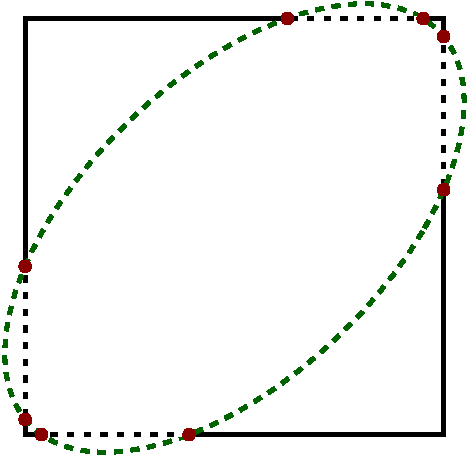
\includegraphics[width=0.3\textwidth]{images/frechet_distance/square-ellipse-intersection.pdf}
  \caption[Legal intervals on free space cell boundary]{
    Legal intervals on the boundaries of a free space cell are shown with black white dashed lines. 
    There are at most 8 intersection points for an ellipse and a rectangle. (Figure inspired by \cite{alt_computing_1995})}
  \label{fig_legal_boundary_intervals_of_a_cell}
\end{figure}

Due to the constant number of intersection points required per cell, 
the free space of a single cell can be computed in $\mathcal{O}(1)$ time.
Therefore, the complete free space of all cells can be computed in $\mathcal{O}(pq)$ time
because there are $p-1$ (respectively $q-1$) edges in $P$ (respectively $Q$).

We observe that there exists 
a monotonically increasing curve from $(0,0)$ to $(p,q)$ in $F_\varepsilon$
if and only if the Fréchet distance between $P$ and $Q$ is less than or equal to $\varepsilon$,
i.e., $\delta_F(P,Q) \leq \varepsilon$.
Given such a curve, the walking speed functions $\alpha$ and $\beta$ from \autoref{def_frechet_distance}
can be easily obtained by rescaling the parameter ranges. 
Computing such a monotonically increasing curve can be done using dynamic programming 
by computing the bottom left most reachable points in each cell starting at $(0,0)$. 
In each step the solution for a single cell can be computed in constant time based on the 
solutions to previously computed cells. 
Therefore, the runtime is also $\mathcal{O}(pq)$. 
See \autoref{fig_free_space_curve} for an example curve. \cite{alt_computing_1995}

\begin{figure}[ht]
  \centering
  \resizebox{0.5\textwidth}{!}{
    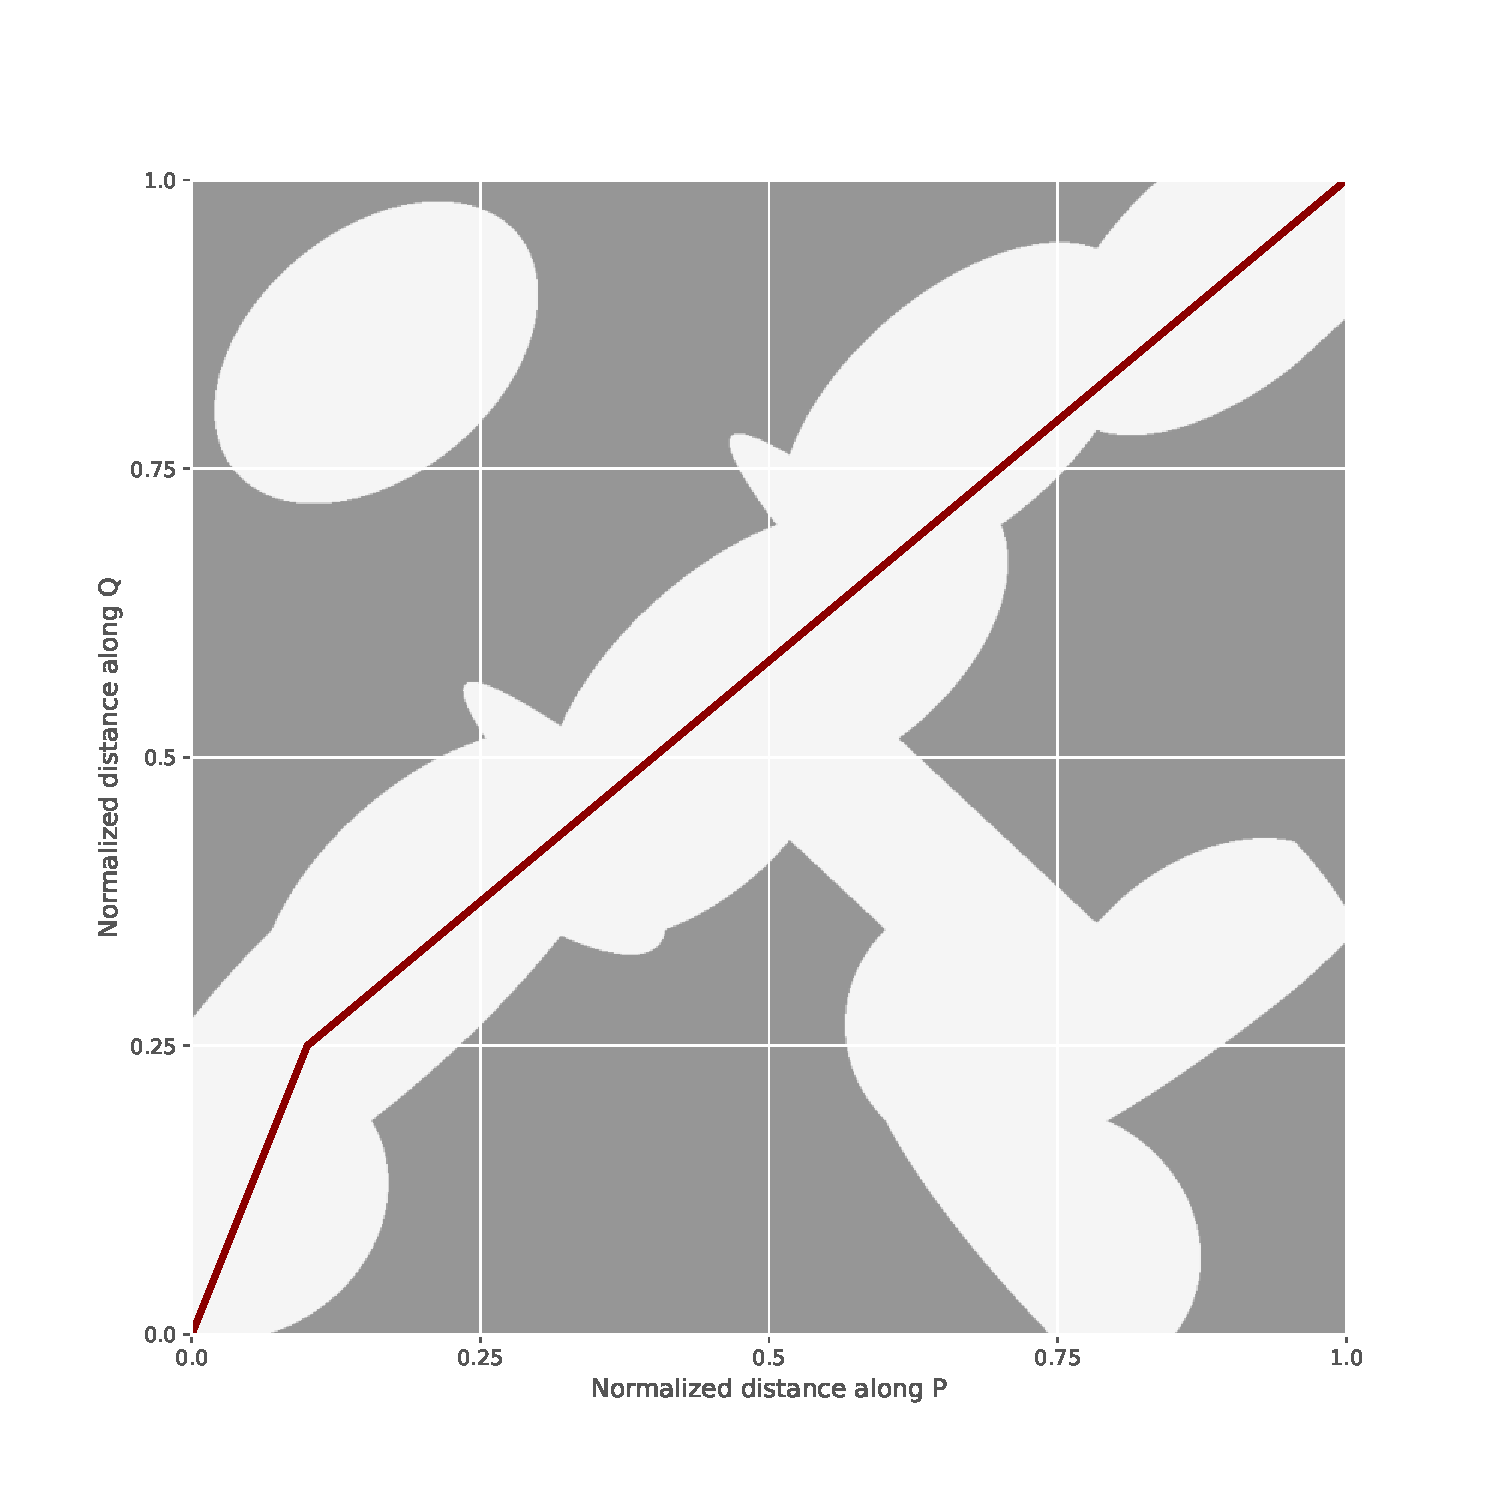
\includegraphics[width=\textwidth]{images/frechet_distance/free_space_monotone_curve.pdf}
    % % This file was created with tikzplotlib v0.10.1.
\begin{tikzpicture}

\definecolor{darkred}{RGB}{139,0,0}
\definecolor{dimgray85}{RGB}{85,85,85}
\definecolor{gainsboro229}{RGB}{229,229,229}

\begin{axis}[
axis background/.style={fill=gainsboro229},
axis line style={white},
height=\textwidth,
minor xtick={},
minor ytick={},
tick align=outside,
tick pos=left,
width=\textwidth,
x grid style={white},
xlabel=\textcolor{dimgray85}{s value used for P(s)},
xmajorgrids,
xmin=-0.5, xmax=4995.5,
xtick style={color=dimgray85},
xtick={0,999,1998,2997,3996,4995},
xticklabels={0,1,2,3,4,5},
y grid style={white},
ylabel=\textcolor{dimgray85}{t value used for Q(t)},
ymajorgrids,
ymin=-0.5, ymax=4995.5,
ytick style={color=dimgray85},
ytick={0,999,1998,2997,3996,4995},
yticklabels={0,1,2,3,4,5}
]
\addplot graphics [includegraphics cmd=\pgfimage,xmin=-0.5, xmax=4995.5, ymin=4995.5, ymax=-0.5] {images/frechet_distance/free_space_monotone_curve_image.png};
\addplot [very thick, darkred]
table {%
0 0
1000 2500
3000 4500
4996 4996
};
\end{axis}

\end{tikzpicture}

  }
  \caption{A monotonically increasing curve (red) through the free space diagram. 
    (Figure inspired by \cite{buchin_four_2017})}
  \label{fig_free_space_curve}
\end{figure}

% Actually computing the exact Fréchet distance
So far we discussed the decision problem whether $\delta_{F}(P,Q) \leq \varepsilon$
and observe that it is solvable in $\mathcal{O}(pq)$ time.
What we actually want to know is the exact value of the Fréchet distance.
A straight forward approach for this is to compute the value bit by bit 
using binary search in total $\mathcal{O}(pq \log (\text{``accuracy''})) = \mathcal{O}(pq  (\text{``accuracy bits''}))$ time.
In practice this approach works really well 
and is often favored over other more complicated approaches. \cite{alt_computing_1995} 

Another approach is to check all values of $\varepsilon$ where something ``interesting'' happens
until the smallest value of $\varepsilon$ is obtained where a monotonically increasing path 
from $(0,0)$ to $(p,q)$ in $F_\varepsilon$ exists.
We will call these the \textit{critical values} of $\varepsilon$, which are:
\begin{enumerate}
  \item the minimal value of $\varepsilon$ where $(0,0) \in F_\varepsilon$ and $(p,q) \in F_\varepsilon$.
  \item values of $\varepsilon$ where a new passage on the border edge 
        between two neighboring cells opens up.
  \item values of $\varepsilon$ where a new horizontal (respectively vertical) passage 
        between two non-neighboring cells opens up.
\end{enumerate}

There is one value of case 1, 
specifically the maximum of starting point to starting point and endpoint to endpoint distance,
$\mathcal{O}(pq)$ values of case 2, 
namely the number of vertex to edge distances,
and $\mathcal{O}(p^2q + pq^2)$ values of case 3,
particularly the number of times two vertices of one curve have the same distance to one edge of the other curve.
Determining all these values can be done in $\mathcal{O}(p^2q + pq^2)$ time 
because each value in each case can be computed in constant time, 
making the values of the third case dominate the time complexity.
% TODO: why does this simplyfication work
These values need to be sorted in $\mathcal{O}((p^2q + pq^2) \log (p^2q + pq^2)) = \mathcal{O}((p^2q + pq^2) \log (pq))$ time
in order to perform binary search in $\mathcal{O}(pq \log (p^2q + pq^2))$ time on them
using the algorithm for the decision problem.
The overall time required for this approach is dominated by the sorting step, 
thus $\mathcal{O}((p^2q + pq^2) \log (pq))$.
This time complexity can be decreased to $\mathcal{O}(pq \log (pq))$ 
using parametric search \cite{megiddo_applying_1983, cole_slowing_1987} to work faster in theory.
However, due to the specific internally used sorting network 
it is hard to implement this efficiently in practice. \cite{alt_computing_1995}



% Runtime analysis (?)
% Correctness proof (?)6

% \subsection{Improved Version?}
% \label{sec_improved_algorithm}
% \cite{van_leusden_novel_2013}
% \cite{buchin_four_2017}


% Algorithms for different variants
\subsection{Algorithm for the Weak Fréchet Distance}
\label{sec_weak_algorithm}
For the weak Fréchet distance, as described in \autoref{sec_weak_frechet_distance},
the computation becomes less complex compared to the continuous Fréchet distance.
Specifically, we can ignore critical values of the third type, 
since it is no longer required to move monotonically 
and one could just go left or down in the free space diagram taking any arbitrary continuous path.
Therefore, the focus shifts towards critical values of the second type, 
those where new passages between neighboring cells open up.
Alt and Godau \cite{alt_computing_1995} proposed two algorithms to compute the weak Fréchet distance.

For both algorithms the problem is modeled as a grid based graph of $p$ by $q$ vertices, 
one for each cell of the free space diagram,
and edges connecting the vertices with their neighboring vertices.
There may be up to four neighboring vertices, namely, 
top, bottom, left, and right.
Additionally, $s$ is added as the start vertex and $t$ as the end vertex.
This results in an undirected Graph $G=(V,E)$ 
where $V = \{C_{i,j} \ | \ 0 \leq i \leq p, 0 \leq j \leq q \} \cup \{s,t\}$
and $E=\{(C_{i,j}, C_{i+1,j}) \ | \ \ 0 \leq i < p, 0 \leq j \leq q\} \cup \{(C_{i,j}, C_{i,j+1}) \ | \ \ 0 \leq i \leq p, 0 \leq j < q\} \cup \{(s, C_{0,0}), (C_{p,q}, t)\}$.
Each edge $(C_{i,j}, C_{i',j'})$ is assigned a critical minimal value of $\varepsilon$ 
such that there is a passage through the border between two cells in the free space. 
Furthermore, the minimal value of $\varepsilon$ such that $(0,0) \in F_\varepsilon$ is assigned to the first edge $(s, C_{0,0})$ 
and the minimal value of $\varepsilon$ such that $(p,q) \in F_\varepsilon$ is assigned to the last edge $(C_{p,q}, t)$. \cite{alt_computing_1995}

The first algorithm is again based on first solving the decision problem 
and then searching for the right $\varepsilon$ through binary search.
The decision problem is satisfied, if and only if there exists a path from $s$ to $t$ in $G$ 
with a maximum single edge value of $\varepsilon$.
This can be checked by removing all edges with values greater than $\varepsilon$ from $E$ 
and then checking if $s$ is still connected to $t$. 
This can be done through some graph traversal algorithm like breadth-first search or depth-first search
in $\mathcal{O}(pq)$ time. \cite{alt_computing_1995}
Since the number of critical values is no longer dominated by the third case,
rather by the second case of $\mathcal{O}(pq)$ values, 
the overall computation problem can be solved in $\mathcal{O}(pq \log (pq))$ time using binary search \cite{van_leusden_novel_2013}. 

The second algorithm works by directly searching for a path from $s$ to $t$ in $G$,
without any prior removal of edges from $E$.
This can be done using Prim's minimum spanning tree algorithm \cite{prim_shortest_1957} starting at $s$ 
and stopping as soon as $t$ is included in the spanning tree. 
The value of $\varepsilon$ is the maximum value of all edged added to the spanning tree.
Similarly, one can use Dijkstra's algorithm \cite{dijkstra_note_1959}, 
optimizing for the minimum maximum edge value.
Both approaches result in a time complexity of $\mathcal{O}(pq \log (pq))$. \cite{alt_computing_1995}
In this case of a planar grid based graph with non-negative edge values 
an even faster algorithm from Henzinger et al. \cite{henzinger_faster_1997} to solve the single source shortest paths problem 
can be applied. This gives a time complexity of $\mathcal{O}(pq)$ to compute the weak Fréchet distance \cite{van_leusden_novel_2013}.


\subsection{Algorithm for the Discrete Fréchet Distance}
\label{sec_discrete_algorithm}
The computation of the discrete Fréchet distance, as defined in \autoref{def_discrete_frechet_distance}, is very easy and straight forward 
using a dynamic programming approach as originally suggested by Eiter et al. \cite{eiter_computing_1994}.
Recall that the polygonal curves $P = (u_1, \dots, u_p)$ and $Q = (v_1, \dots, v_p)$ are defined as sequences of points.
The algorithm works by recursively computing the minimal required $\varepsilon$ for partial curves 
$P' = (u_1, \dots, u_i)$ and $Q' = (v_1, \dots, v_j)$
using $c(i,j)$ as defined in \autoref{def_recursive_forumla_discrete_frechet_distance}.
Starting from $c(1,1)$, which is the distance between the starting points $u_1$ and $v_1$,
all other values of $c(i,j)$ are computed iteratively in a bottom up manner 
with memoization on the previously computed values of $c(i,j)$.
The resulting algorithm has runtime of $\mathcal{O}(pq)$
because the constant time function $c(i,j)$ is called $pq$ times \cite{eiter_computing_1994}.
Additionally, the algorithm can be implemented to require $\mathcal{O}(min(p,q))$ space 
because it is sufficient to store the previous column or row of $c(i,j)$ values 
for memoization.

\begin{mydef}
  \label{def_recursive_forumla_discrete_frechet_distance}
  The discrete Fréchet distance of the two (partial) polygonal curves $P' = (u_1, \dots, u_i)$ and $Q' = (v_1, \dots, v_j)$
  can be computed by
  \begin{align*}
    c(i,j) &= \begin{cases}
      dist(u_1, v_1), &\text{if } i=1 \text{and } j=1 \\
      \max \{c(i-1,1), dist(u_i, v_1)\}, &\text{if } i>1 \text{and } j=1 \\
      \max \{c(1,j-1), dist(u_1, v_j)\}, &\text{if } i=1 \text{and } j>1 \\
      \max \{c(i-1,j), c(i,j-1), c(i-1,j-1), dist(u_i, v_j)\}, &\text{if } i>1 \text{and } j>1
    \end{cases} \\
    &= \delta_{dF}(P',Q')
  \end{align*}
\end{mydef}

\section{Conclusion}
% Which version to use when
This work gives an overview on the Fréchet distance, 
its variants and algorithms to compute them. 
Several differences between the variants have been described 
and evaluated. 
In conclusion, it can be stated that computing the continuous 
Fréchet distance is more computationally expensive compared 
to its discrete and weak variants.
However, computing the continuous variant can be done efficiently
in practice by binary searching the bits of the desired accuracy directly
instead of computing the formally correct value. 
Alternatively, the discrete Fréchet distance can be calculated, 
since it bounds the continuous distance 
from below and above. 
In this way, the tolerance range can be narrowed down to a desired size.




%%%
%%% end main document
%%%
%%%%%%%%%%%%%%%%%%%%%%%%%%%%%%%%%%%%%%%%%%%%%%%%%%%%%%%%%%%%%%%%%%%%%%%%%%%%%%%%

\newpage
\appendix  %% include it, if something (bibliography, index, ...) follows below

%%%%%%%%%%%%%%%%%%%%%%%%%%%%%%%%%%%%%%%%%%%%%%%%%%%%%%%%%%%%%%%%%%%%%%%%%%%%%%%%
%%%
%%% bibliography
%%%
%%% available styles: abbrv, acm, alpha, apalike, ieeetr, plain, siam, unsrt
%%%
\bibliographystyle{alpha}

%%% name of the bibliography file without .bib
%%% e.g.: literature.bib -> \bibliography{literature}
\bibliography{literature}

\end{document}
%%% }}}
%%% END OF FILE
